% !TEX root =index.tex
\setchapterpreamble[u]{\margintoc}
\chapter{Proof-by-Action in Practice}
\labch{advanced}

\epigraph{Practical life is not necessarily directed toward other people, as
some think; and it is not the case that practical thoughts are only those which
result from action for the sake of what ensues. On the contrary, much more
practical are those mental activities and reflections which have their goal in
themselves and take place for their own sake.}{\textbf{Aristotle},
\textit{Politics, VII, 3, 8, 1325b16-20}}

In the previous chapters, we explained the core principles of our so-called
\kl{Proof-by-Action} paradigm and especially of its drag-and-drop actions, first
through basic and abstract examples in \refch{pba}, and then from a
\kl{proof-theoretical} perspective in \refch{sfl}. The goal of this chapter is
to provide a better sense of what proofs by action/\kl{DnD} look like in
practice, and how they compare to more traditional approaches to interactive
theorem proving. To that effect, we perform a case study of a few select
examples, unrolling and commenting in details one or many of their proofs.
Although still basic, they are fully fledged, concrete logical riddles or
mathematical problems that one might give as exercise to an undergraduate
student learning formal proofs. Note that our analysis will stay quite informal
and opinionated: a more systematic approach such as a user study would allow for
a better evaluation of our paradigm, but at the time of writing of this thesis
the \kl{Actema} prototype is not mature enough to conduct a project of this
scale.

The chapter is organized as follows: \refsec{edukera} studies a proof of a small
logical riddle in \kl{Actema}, highlighting some benefits of our approach
compared to textual systems. \refsec{funcs} explores how basic properties about
functions between sets can be proved graphically, introducing the use of
\emph{definitions} in addition to logical reasoning steps. In \refsec{arith} we
prove equations in Peano arithmetic, showing how one can incorporate additional
actions into the paradigm to deal with more specialized forms of reasoning:
\emph{induction} and \emph{automatic computation}.

\begin{kaonote}
  For each example, we provide a \kl{Coq} \kl{proof script} that tries to follow
  the structure of the graphical proof, for the sake of comparison with a
  textual interface. But this would obviously compare differently with other
  textual interfaces, like the \kl{Isar} proof language which is more
  declarative, and thus farther from the imperative aspects of \kl{PbA}.
\end{kaonote}
  
\section{Forward reasoning}\labsec{edukera}

% It is too early to perform a detailed case study comparing our approach
% to interactive theorem proving with others --- tactic-based,
% declarative, {\em etc}\dots~This is due primarily to the fact that
% our prototype is not mature enough; it cannot handle lemmas and
% implements a limited formalism. However some examples allow to get a
% glimpse of specificities and possible advantages of proofs by actions.

\subsection{A gestural proof}

\AP
Our first example is a small logical riddle, which we borrow from a textual
educational system, \intro{Edukera}~\sidecite{edukera}. We invite readers to try
to perform the proof themselves in the online version of
\kl{Actema}\sidenote{\url{https://www.actema.xyz/courses/edukera}}. One
considers a population of people, with at least one individual $h$, together
with a single function $\mother$ and one predicate $\rich$. The aim is to show
that the two following assumptions are incompatible:
\begin{gather}
  \forall x. \neg\rich(x)\lor \neg\rich(\mother(\mother(x))) \label{hyp:1} \\
  \forall x. \neg\rich(x) \limp \rich(\mother(x)) \label{hyp:2}
\end{gather}
The original \kl{goal} thus corresponds to the illustration of \reffig{edukera}.

\begin{figure*}
  \fbox{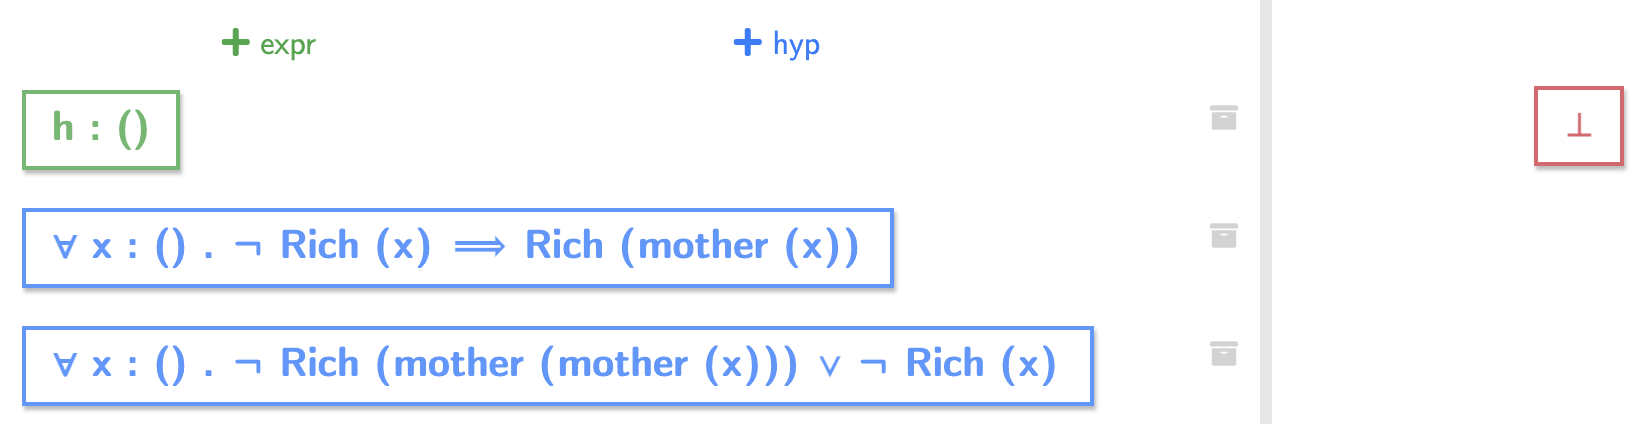
\includegraphics[width=1.3\textwidth]{edukera.png}}
  \caption{The beginning of an example due to \kl{Edukera}}
  \labfig{edukera}
\end{figure*}

It is quite natural to approach this problem in a \kl{forward} manner, by
starting from the hypotheses to establish new facts. And a first point
illustrated by this example is that \kl{DnD} actions allow to do this in a
smooth and precise manner. A possible first step is to bring $h$ to
hypothesis~(\ref{hyp:1}), to obtain a new fact:
\begin{gather}
  ~\neg\rich(h)\lor \neg\rich(\mother(\mother(h))) \label{hyp:3}
\end{gather}
Double-clicking on this new fact yields two cases:
\begin{gather}
  \neg\rich(h) \label{hyp:4} \\
  \neg\rich(\mother(\mother(h))) \label{hyp:5}
\end{gather}
Let us detail how one solves the second one. By bringing
hypothesis~(\ref{hyp:5}) on the premise of hypothesis~(\ref{hyp:2}) one obtains
\begin{gather}
  \rich(\mother(\mother(\mother(h)))) \label{hyp:6}
\end{gather}
The next step is a good example where \kl{DnD} actions are useful. By bringing
this new fact to the right-hand part of hypothesis~(\ref{hyp:3}) one immediately
obtains a new fact
\begin{gather}
  \neg{\rich(\mother(h))} \label{hyp:7}
\end{gather}
In textual proof languages, this last step requires a somewhat intricate
\kl{tactic} line and/or writing down at least the statement of the new fact.

One can then finish the case by combining hypotheses (\ref{hyp:7}) and
(\ref{hyp:2}), which yields
$$\rich(\mother(\mother(h)))$$
contradicting hypothesis~(\ref{hyp:5}). These two last steps each correspond to a
simple \kl{DnD}. The other case, $\neg\rich(h)$, is quite similar.

% Such a simple example is not sufficient to provide significant metrics.
Note that once a user has understood the proof, the riddle is routinely solved
in less than a minute in \kl{Actema}, which seems out of reach for about any user in
a \kl{tactic}-based prover. At least as important is the fact that the proof can be
performed without typing any text, especially no intermediate statement. 

\subsection{Comparison with a textual proof}

To conclude this example, we propose in \reffig{edukera-coq} a complete proof of
the riddle formalized in the \kl{Coq} \kl{proof assistant}, which follows very closely the
structure of the graphical proof just outlined. To make the correspondence more
visible and ease the comparison, we interspersed the \kl{proof script} with comments
of the form \texttt{(** [actions] *)}, where \texttt{[actions]} is a
sentence describing a sequence of actions in \kl{Actema} that produces the same goal
transformation as the \kl{tactics} preceding the comment. There are a few interesting
things to note:
\begin{description}
  \item[Hypotheses management] We chose to name manually all the hypotheses
  introduced in the course of the proof. This is generally considered good
  practice in the \kl{Coq} community, because it makes \kl{proof scripts} easier
  to maintain. In our case it also has the advantage of expliciting which
  hypotheses are used exactly in the reasoning, something that an \kl{Actema}
  user does with her pointing device when designating the blue \kl{items}
  involved in an action.
  
  It appears clearly in \reffig{edukera-coq} that in a moderately long proof
  like this based mostly on \kl{forward} reasoning, one needs to keep track of
  \emph{a lot} of names, which can be overwhelming for many users. This is
  especially true for beginners discovering \kl{Coq}, because the syntax for
  assigning names, based on patterns like \texttt{[H | H]} that reproduce the
  \kl{subgoal} structure, can induce a steep learning curve. Of course this
  problem is mitigated trivially in \kl{Actema}, since names are not needed.

  \item[Tactics vs. actions] There is no exact correspondence between the
  \kl{tactics} of \kl{Coq} and the actions of \kl{Actema}: some \kl{tactics} are
  simulated by multiple actions, and often a complex sequence of \kl{tactics}
  can be simulated by a single action\sidenote{This was already noticed in
  \cite{PbP}, where clicking on a subformula can simulate a sequence of
  \kl{introduction rules} of arbitrary length.}.
  
  For instance, line 23 does at the same time a specialization of the hypothesis
  $H_2 : \forall x. \neg \rich(\mother(\mother(x))) \lor \neg \rich(x)$ to the
  individual $h$ with the application \texttt{(H2 h)}, and a case analysis with
  the \texttt{destruct} \kl{tactic}. In \kl{Actema} this is performed in two steps, first
  by drag-and-dropping $h$ on $H_2$, and then by clicking on the resulting
  hypothesis\sidenote{This could also be achieved in two steps in \kl{Coq}, by using
  the \texttt{specialize} \kl{tactic} instead of the inlined application.}.

  In the other direction, a pattern of reasoning that occurs multiple times in
  the proof is the combination of $H_2$ with another hypothesis which
  contradicts one of the two cases, in order to deduce the truth of the other
  case. While it is captured straightforwardly in \kl{Actema} with a single \kl{DnD}
  between the contradictory statements, it requires in \kl{Coq} a decomposition into
  many administrative steps:
  \begin{enumerate}
    \item first a case analysis with \texttt{destruct}, where the expression
    instantiating $H_2$ (e.g. $\mother(\mother(h))$) needs to be written down
    explicitly, instead of being inferred automatically from unification;
    \item optionally focusing on the \kl{subgoal} corresponding to the contradictory
    case if it is the right disjunct (line 56), which requires to know a
    somewhat idiosyncratic and infrequently used syntax of the \kl{tactic} language;
    \item and finally expliciting the contradiction with \texttt{apply} and
    \texttt{exact}.
  \end{enumerate}

  \item[Context-sensitivity] More generally, the actions of \kl{Actema} are more
  \emph{versatile} and \emph{context-aware} than the \kl{tactics} of \kl{Coq}.
  For instance, click actions have a different effect depending on the main
  connective of the formula being clicked, but provide a unique interface for
  applying rules of natural deduction/\kl{sequent calculus}. On the contrary,
  there is almost one \kl{tactic} for dealing with each logical connective in
  \kl{Coq}, e.g. \texttt{intros} for $\limp$ and $\forall$, \texttt{split} for
  $\land$, \texttt{left} and \texttt{right} for $\lor$, \texttt{exists} for
  $\exists$, etc. The same remark applies to \kl{DnD} actions, whose
  functionalities are provided in \kl{Coq} by many different \kl{tactics}:
  \texttt{apply \_}, \texttt{apply \_ in \_}, \texttt{pose proof},
  \texttt{specialize}, etc.
\end{description}

\begin{figure}
  % \fontsize{8}{8.5}\selectfont
  % \begin{alectryon}
  % Generator: Alectryon
  \sep
  \begin{txt}
    \PY{c}{(*~Declaration~of~constants~used~in~the~statement~of~the~riddle~*)}\nl
    \nl
  \end{txt}
  \sep
  \begin{sentence}
    \begin{input}
      \PY{k+kn}{Context}~\PY{o}{(}\PY{n+nv}{i}~\PY{o}{:}~\PY{k+kt}{Type}\PY{o}{).}\nl
    \end{input}
  \end{sentence}
  \sep
  \begin{txt}
    \nl
  \end{txt}
  \sep
  \begin{sentence}
    \begin{input}
      \PY{k+kn}{Context}~\PY{o}{(}\PY{n+nv}{Rich}~\PY{o}{:}~\PY{n}{i}~\PY{o}{\PYZhy{}\PYZgt{}}~\PY{k+kt}{Prop}\PY{o}{).}\nl
    \end{input}
  \end{sentence}
  \sep
  \begin{sentence}
    \begin{input}
      \PY{k+kn}{Context}~\PY{o}{(}\PY{n+nv}{mother}~\PY{o}{:}~\PY{n}{i}~\PY{o}{\PYZhy{}\PYZgt{}}~\PY{n}{i}\PY{o}{).}\nl
    \end{input}
  \end{sentence}
  \sep
  \begin{sentence}
    \begin{input}
      \PY{k+kn}{Context}~\PY{o}{(}\PY{n+nv}{h}~\PY{o}{:}~\PY{n}{i}\PY{o}{).}\nl
    \end{input}
  \end{sentence}
  \sep
  \begin{txt}
    \nl
    \PY{c}{(*~Statement~of~the~riddle~*)}\nl
    \nl
  \end{txt}
  \sep
  \begin{sentence}
    \begin{input}
      \PY{k+kn}{Theorem}~\PY{n+nf}{rich\PYZus{}mothers}~\PY{o}{:}\nl
      ~~\PY{o}{(}\PY{k+kr}{forall}~\PY{n+nv}{x}\PY{o}{,}~\PY{o}{\PYZti{}}\PY{n}{Rich}\PY{o}{(}\PY{n}{x}\PY{o}{)}~\PY{o}{\PYZhy{}\PYZgt{}}~\PY{n}{Rich}\PY{o}{(}\PY{n}{mother}\PY{o}{(}\PY{n}{x}\PY{o}{)))}~\PY{o}{\PYZhy{}\PYZgt{}}\nl
      ~~\PY{o}{(}\PY{k+kr}{forall}~\PY{n+nv}{x}\PY{o}{,}~~\PY{o}{\PYZti{}}\PY{n}{Rich}\PY{o}{(}\PY{n}{mother}\PY{o}{(}\PY{n}{mother}\PY{o}{(}\PY{n}{x}\PY{o}{)))}~\PY{o}{\PYZbs{}/}~\PY{o}{\PYZti{}}\PY{n}{Rich}\PY{o}{(}\PY{n}{x}\PY{o}{))}~\PY{o}{\PYZhy{}\PYZgt{}}\nl
      ~~\PY{k+kt}{False}\PY{o}{.}\nl
    \end{input}
  \end{sentence}
  \sep
  \begin{txt}
    \nl
    \PY{c}{(*~Proof~of~the~riddle~*)}
  \end{txt}
\end{alectryon}

\begin{alectryon}
  % Generator: Alectryon
  \sep
  \begin{sentence}
    \begin{input}
      \PY{k+kn}{Proof}\PY{o}{.}\nl
    \end{input}
  \end{sentence}
  \sep
  \begin{sentence}
    \begin{input}
      ~~\PY{n+nb}{intros}~\PY{n}{H1}~\PY{n}{H2}\PY{o}{.}\nl
    \end{input}
  \end{sentence}
  \sep
  \begin{txt}
    \nl
    ~~\PY{l+s+sd}{(**~2~clicks~on~the~conclusion~*)}\nl
    \nl
  \end{txt}
  \sep
  \begin{sentence}
    \begin{input}
      ~~\PY{n+nb}{destruct}~\PY{o}{(}\PY{n}{H2}~\PY{n}{h}\PY{o}{)}~\PY{k+kr}{as}~\PY{o}{[}\PY{n}{H}~\PY{o}{|}~\PY{n}{H}\PY{o}{].}\nl
    \end{input}
  \end{sentence}
  \sep
  \begin{txt}
    \nl
    ~~\PY{l+s+sd}{(**~DnD~of~[h]~onto~[H2],~then~click~on~the~resulting~hypothesis~*)}\nl
    \nl
  \end{txt}
  \sep
  \begin{sentence}
    \begin{input}
      ~~\PY{o}{*}~
    \end{input}
  \end{sentence}
  \sep
  \begin{sentence}
    \begin{input}
      \PY{n+nb}{pose~proof}~\PY{o}{(}\PY{n}{H1}~\PY{n}{\PYZus{}}~\PY{n}{H}\PY{o}{)}~\PY{k+kr}{as}~\PY{n}{H\PYZsq{}}\PY{o}{.}\nl
    \end{input}
  \end{sentence}
  \sep
  \begin{txt}
    \nl
    ~~~~\PY{c}{(*~If~one~naively~uses~[apply~\PYZus{}~in],~then~one~loses~[H]~although}\nl
    \PY{c}{~~~~~~~it~is~needed~later!~Hence~the~use~of~[pose~proof].~*)}\nl
    \nl
    ~~~~\PY{l+s+sd}{(**~DnD~of~[H1]~onto~[H]~*)}\nl
    \nl
  \end{txt}
  \sep
  \begin{sentence}
    \begin{input}
      ~~~~\PY{n+nb}{destruct}~\PY{o}{(}\PY{n}{H2}~\PY{o}{(}\PY{n}{mother}~\PY{n}{h}\PY{o}{))}~\PY{k+kr}{as}~\PY{o}{[}\PY{n}{H2\PYZsq{}}~\PY{o}{|}~\PY{n}{H2\PYZsq{}}\PY{o}{].}\nl
    \end{input}
  \end{sentence}
  \sep
  \begin{sentence}
    \begin{input}
      ~~~~\PY{n+nb}{apply}~\PY{n}{H2\PYZsq{}}\PY{o}{.}~
    \end{input}
  \end{sentence}
  \sep
  \begin{sentence}
    \begin{input}
      \PY{n+nb+bp}{exact}~\PY{n}{H\PYZsq{}}\PY{o}{.}\nl
    \end{input}
  \end{sentence}
  \sep
  \begin{txt}
    \nl
    ~~~~\PY{l+s+sd}{(**~DnD~of~[H\PYZsq{}]~onto~[H2].~Could~also~be~performed~stepwise:~~}\nl
    \PY{l+s+sd}{~~~~~~~~\PYZhy{}~Selection~of~[mother(h)]~in~[H\PYZsq{}]}\nl
    \PY{l+s+sd}{~~~~~~~~\PYZhy{}~DnD~of~[H\PYZsq{}]~onto~[H2]}\nl
    \PY{l+s+sd}{~~~~~~~~\PYZhy{}~Click~on~the~resulting~hypothesis}\nl
    \PY{l+s+sd}{~~~~~~~~\PYZhy{}~DnD~of~[H2\PYZsq{}]~onto~[H\PYZsq{}]~*)}\nl
    \nl
  \end{txt}
  \sep
  \begin{sentence}
    \begin{input}
      ~~~~\PY{n+nb}{apply}~\PY{n}{H1}~\PY{k+kr}{in}~\PY{n}{H2\PYZsq{}}\PY{o}{.}\nl
    \end{input}
  \end{sentence}
  \sep
  \begin{txt}
    \nl
    ~~~~\PY{l+s+sd}{(**~DnD~of~[H1]~onto~[H2\PYZsq{}]~*)}\nl
    \nl
  \end{txt}
  \sep
  \begin{sentence}
    \begin{input}
      ~~~~\PY{n+nb}{apply}~\PY{n}{H}\PY{o}{.}~
    \end{input}
  \end{sentence}
  \sep
  \begin{sentence}
    \begin{input}
      \PY{n+nb+bp}{exact}~\PY{n}{H2\PYZsq{}}\PY{o}{.}\nl
    \end{input}
  \end{sentence}
  \sep
  \begin{txt}
    \nl
    ~~~~\PY{l+s+sd}{(**~DnD~of~[H]~onto~[H2\PYZsq{}]~*)}\nl
    \nl
  \end{txt}
  \sep
  \begin{sentence}
    \begin{input}
      ~~\PY{o}{*}~
    \end{input}
  \end{sentence}
  \sep
  \begin{sentence}
    \begin{input}
      \PY{n+nb}{pose~proof}~\PY{o}{(}\PY{n}{H1}~\PY{n}{\PYZus{}}~\PY{n}{H}\PY{o}{)}~\PY{k+kr}{as}~\PY{n}{H\PYZsq{}}\PY{o}{.}\nl
    \end{input}
  \end{sentence}
  \sep
  \begin{txt}
    \nl
    ~~~~\PY{l+s+sd}{(**~DnD~of~[H1]~onto~[H]~*)}\nl
    \nl
  \end{txt}
  \sep
  \begin{sentence}
    \begin{input}
      ~~~~\PY{n+nb}{destruct}~\PY{o}{(}\PY{n}{H2}~\PY{o}{(}\PY{n}{mother}~\PY{n}{h}\PY{o}{))}~\PY{k+kr}{as}~\PY{o}{[}\PY{n}{H2\PYZsq{}}~\PY{o}{|}~\PY{n}{H2\PYZsq{}}\PY{o}{].}\nl
    \end{input}
  \end{sentence}
  \sep
  \begin{sentence}
    \begin{input}
      ~~~~\PY{l+m+mi}{2}\PY{o}{:}~\PY{o}{\PYZob{}}~
    \end{input}
  \end{sentence}
  \sep
  \begin{sentence}
    \begin{input}
      \PY{n+nb}{apply}~\PY{n}{H2\PYZsq{}}\PY{o}{.}~
    \end{input}
  \end{sentence}
  \sep
  \begin{sentence}
    \begin{input}
      \PY{n+nb+bp}{exact}~\PY{n}{H\PYZsq{}}\PY{o}{.}~
    \end{input}
  \end{sentence}
  \sep
  \begin{sentence}
    \begin{input}
      \PY{o}{\PYZcb{}}\nl
    \end{input}
  \end{sentence}
  \sep
  \begin{txt}
    \nl
    ~~~~\PY{l+s+sd}{(**~DnD~of~[H\PYZsq{}]~onto~[H2]~*)}\nl
    \nl
  \end{txt}
  \sep
  \begin{sentence}
    \begin{input}
      ~~~~\PY{n+nb}{pose~proof}~\PY{o}{(}\PY{n}{H1}~\PY{n}{\PYZus{}}~\PY{n}{H2\PYZsq{}}\PY{o}{)}~\PY{k+kr}{as}~\PY{n}{H2\PYZsq{}\PYZsq{}}\PY{o}{.}\nl
    \end{input}
  \end{sentence}
  \sep
  \begin{txt}
    \nl
    ~~~~\PY{l+s+sd}{(**~DnD~of~[H1]~onto~[H2\PYZsq{}]~*)}\nl
    \nl
  \end{txt}
  \sep
  \begin{sentence}
    \begin{input}
      ~~~~\PY{n+nb}{destruct}~\PY{o}{(}\PY{n}{H2}~\PY{o}{(}\PY{n}{mother}~\PY{o}{(}\PY{n}{mother}~\PY{n}{h}\PY{o}{)))}~\PY{k+kr}{as}~\PY{o}{[}\PY{n}{H2\PYZsq{}\PYZsq{}\PYZsq{}}~\PY{o}{|}~\PY{n}{H2\PYZsq{}\PYZsq{}\PYZsq{}}\PY{o}{].}\nl
    \end{input}
  \end{sentence}
  \sep
  \begin{sentence}
    \begin{input}
      ~~~~\PY{n+nb}{apply}~\PY{n}{H2\PYZsq{}\PYZsq{}\PYZsq{}}\PY{o}{.}~
    \end{input}
  \end{sentence}
  \sep
  \begin{sentence}
    \begin{input}
      \PY{n+nb+bp}{exact}~\PY{n}{H2\PYZsq{}\PYZsq{}}\PY{o}{.}\nl
    \end{input}
  \end{sentence}
  \sep
  \begin{txt}
    \nl
    ~~~~\PY{l+s+sd}{(**~DnD~of~[H2\PYZsq{}\PYZsq{}]~onto~[H2]~*)}\nl
    \nl
  \end{txt}
  \sep
  \begin{sentence}
    \begin{input}
      ~~~~\PY{n+nb}{apply}~\PY{n}{H1}~\PY{k+kr}{in}~\PY{n}{H2\PYZsq{}\PYZsq{}\PYZsq{}}\PY{o}{.}\nl
    \end{input}
  \end{sentence}
  \sep
  \begin{txt}
    \nl
    ~~~~\PY{l+s+sd}{(**~DnD~of~[H1]~onto~[H2\PYZsq{}\PYZsq{}\PYZsq{}]~*)}\nl
    \nl
  \end{txt}
  \sep
  \begin{sentence}
    \begin{input}
      ~~~~\PY{n+nb}{apply}~\PY{n}{H2\PYZsq{}}\PY{o}{.}~
    \end{input}
  \end{sentence}
  \sep
  \begin{sentence}
    \begin{input}
      \PY{n+nb+bp}{exact}~\PY{n}{H2\PYZsq{}\PYZsq{}\PYZsq{}}\PY{o}{.}\nl
    \end{input}
  \end{sentence}
  \sep
  \begin{txt}
    \nl
    ~~~~\PY{l+s+sd}{(**~DnD~of~[H2\PYZsq{}]~onto~[H2\PYZsq{}\PYZsq{}\PYZsq{}]~*)}\nl
  \end{txt}
  \sep
  \begin{sentence}
    \begin{input}
      \PY{k+kn}{Qed}\PY{o}{.}
    \end{input}
  \end{sentence}
\end{alectryon}
  \begin{minted}
  [
  frame=lines,
  framesep=2mm,
  baselinestretch=1,
  fontsize=\footnotesize,
  linenos
  ]
  {coq}

(* Declaration of constants used in the statement of the riddle *)

Context (i : Type).
Context (Rich : i -> Prop).
Context (mother : i -> i).
Context (h : i).

(* Statement of the riddle *)

Theorem rich_mothers :
  (forall x, ~Rich(x) -> Rich(mother(x))) ->
  (forall x,  ~Rich(mother(mother(x))) \/ ~Rich(x)) ->
  False.

(* Proof of the riddle *)

Proof.
  intros H1 H2.
  (** 2 clicks on the conclusion *)

  destruct (H2 h) as [H | H].
  (** DnD of [h] onto [H2], then click on the resulting hypothesis *)

  * pose proof (H1 _ H) as H'.
    (* If one naively uses [apply _ in], then one loses [H] although
       it is needed later! Hence the use of [pose proof]. *)
    (** DnD of [H1] onto [H] *)
    
    destruct (H2 (mother h)) as [H2' | H2'].
    apply H2'. exact H'.
    (** DnD of [H'] onto [H2]. Could also be performed stepwise:  
        - Selection of [mother(h)] in [H']
        - DnD of [H'] onto [H2]
        - Click on the resulting hypothesis
        - DnD of [H2'] onto [H'] *)

    apply H1 in H2'.
    (** DnD of [H1] onto [H2'] *)

    apply H. exact H2'.
    (** DnD of [H] onto [H2'] *)

  * pose proof (H1 _ H) as H'.
    (** DnD of [H1] onto [H] *)

    destruct (H2 (mother h)) as [H2' | H2'].
    2: { apply H2'. exact H'. }
    (** DnD of [H'] onto [H2] *)

    pose proof (H1 _ H2') as H2''.
    (** DnD of [H1] onto [H2'] *)

    destruct (H2 (mother (mother h))) as [H2''' | H2'''].
    apply H2'''. exact H2''.
    (** DnD of [H2''] onto [H2] *)

    apply H1 in H2'''.
    (** DnD of [H1] onto [H2'''] *)

    apply H2'. exact H2'''.
    (** DnD of [H2'] onto [H2'''] *)
Qed.

\end{minted}
  \caption{\kl{Coq} \kl{proof script} formalizing \kl{Edukera}'s riddle}
  \labfig{edukera-coq}
\end{figure}

From this detailed comparison, it appears that the interface offered by the
\kl{PbA} paradigm might be more suited to \kl{forward} reasoning than the
\kl{tactic} language of \kl{Coq}, at least in some respects. It makes the flow of
argumentation more straightforward to express with \kl{DnD} actions, and avoids the
overheads of name management and syntax memorization. This altogether shall
prove to be particularly helpful to beginners and learners of the \kl{proof
assistant}.


\section{Sets and functions}\labsec{funcs}

\subsection{A simple exercise}

Our second example comes from a preprint of Bartzia et al.
\sidecite{bartzia:hal-04087080}, where it is chosen specifically for a case
study aiming to compare the features of different \kl{proof assistants}'
interfaces in an educational setting. It is ``a typical exercise about sets,
relations and functions, as commonly found in introductory courses about
reasoning and proof.'' (p.~6):

\begin{exercise}
  Given three sets $A$, $B$ and $C$ such that $C \subseteq A$ and a function $f
  : A \to B$, show that:
  \begin{enumerate}
    \item $C \subseteq f^{-1}(f(C))$.
    \item If $f$ is injective then $f^{-1}(f(C)) \subseteq C$.
  \end{enumerate}
  where $f(D)$ and $f^{-1}(E)$ denote respectively the direct and inverse image
  (or preimage) of sets $D \subseteq A$ and $E \subseteq B$ by $f$.
\end{exercise}

\AP
Compared to our previous example, this exercise has the particularity of
involving multiple \emph{definitions}, here about sets and functions between
them. There are many possible ways to handle definitions in a formal \kl{proof
system}. A common one, which might be termed \intro{nominal}, is to decompose
the definition into a new function or predicate symbol, the definition's
\intro{head}, and a universally parametrized equality or equivalence between the
\kl{head} and the \intro{body} of the definition. For instance, the concept of
injectivity can be encoded as a unary predicate $\injective(\cdot)$ on
functions, satisfying the following equivalence:
$$\forall A.\ \forall B.\ \forall f{:}A \to B.~\ \injective(f) ~\lequiv~ \forall x
\in A.\ \forall y \in A.\ f(x) = f(y) \limp x = y$$
Notice that $\injective(\cdot)$ is a \emph{\kl{higher-order}} predicate, since it
takes any function as argument. Depending on the underlying logical framework,
this might have an impact on the exact way the definition is encoded. Here we do
not want to bother with such implementation details, and simply assume that
\kl{higher-order} definitions are possible, even though \kl{Actema} is currently limited
to \kl{first-order logic}. In practice this does not affect the semantics of
graphical actions, and we can imagine having a \kl{first-order} \kl{set theory} such as
\kl{ZF} to make everything work behind the scenes\sidenote{See also
\refsec{pluginfuture} for a discussion on a \kl{higher-order} extension of \kl{Actema}.}.

\subsection{Nominal definitions}

\AP
Let us now describe how to prove the second question of the exercise in the
\kl{PbA} paradigm. The first thing we want to do is to unfold the definition of
set inclusion in the conclusion $f^{-1}(f(C)) \subseteq C$, so that we can see
how to prove logically such an inclusion. One might imagine multiple kinds of
graphical actions for doing this. In \kl{Actema} we implemented a general
\emph{subterm selection} mechanism, where the user can successively point at
different subterms appearing in the \kl{goal} and then choose from a list of
so-called \intro{contextual actions} that take the selection as argument. In our
case we can select the whole conclusion, and then choose to apply the
\intro{Unfold} action:
$$\select{f^{-1}(f(C)) \subseteq C} \qquad \text{(\kl{Unfold})}$$
The system will be able to tell that we selected an instance of the two-place
inclusion predicate $\cdot \subseteq \cdot$, and thus will replace the \kl{head}
of this definition by its \kl{body}, instantiating parameters accordingly. This
gives us a new conclusion
$$\forall x. x \in f^{-1}(f(C)) \limp x \in C$$
on which we can click twice to introduce a new variable $x$ in the \kl(sequent){context},
together with the new hypothesis
\begin{gather}
  x \in f^{-1}(f(C)) \label{hyp::1}
\end{gather}
Now there is no available action on the conclusion $x \in C$, because set
membership is a \emph{primitive} predicate in \kl{set theory}. But we can still
unfold some definitions in the \kl(sequent){context}, which might suggest
further possible interactions. First we can unfold the definition of preimage
used in hypothesis~(\ref{hyp::1}) by selecting the precise corresponding
subterm:
$$x \in \select{f^{-1}(f(C))} \qquad \text{(\kl{Unfold})}$$
which, assuming a definition based on set comprehension, gives:
\begin{gather}
  x \in \compr{a \in A}{f(a) \in f(C)} \label{hyp::2}
\end{gather}
At this stage, we would like to make the set comprehension in
hypothesis~(\ref{hyp::2}) disappear, by simply deducing $f(x) \in f(C)$ from it.
But depending on the underlying logical framework, the way to perform this
deduction step in \kl{PbA} will vary.

\subsection{Axiomatic definitions}

\AP
In a set theory such as \kl{ZF}, the meaning of $\in$ comes from the various
\kl{axioms} involving it. One might call this a \intro{behavioral} (or
\reintro{axiomatic}) definition, since the meaning of the \kl{symbol} emerges
from the way it can be used in proofs through \kl{axioms}. This contrasts with
the previous \kl{nominal} definitions, that have a much simpler semantics
captured by \kl{Unfold} actions\sidenote{Note that the syntax of
\kl{first-order logic} is unaware of this distinction, since in both cases the
defined concepts are encoded as \emph{atomic} predicates. This is usually not
the case of logical frameworks found in \kl{proof assistants}: for instance, the
duality between \intro{judgmental} (\kl{nominal}) and \emph{propositional}
(\kl{behavioral}) equality is at the heart of \kl{Martin-Löf type theory}, and
it is used extensively in \kl{Coq} to perform automation, both in the
computation of expressions and the matching of statements modulo definitions.}.

In particular, we can simplify the set comprehension in
hypothesis~(\ref{hyp::2}) by invoking explicitly the \emph{axiom of
comprehension}, which states the following:
$$\forall \phi.\ \forall D.\ \forall y.\ y \in \compr{d \in D}{\phi}
~~\lequiv~~ (y \in D \land \subst{\phi}{y}{d})$$
Note that this is again a \kl{higher-order} statement, but this time because it
quantifies over every formula $\phi$\sidenote{Traditionnally, logicians
preferred to speak of \emph{axiom schemas}, that is countable sets of
\kl{axioms}, rather than \kl{higher-order} \kl{axioms}, in order to stay purely
in a \kl{first-order} setting. But this does not make much sense from an
implementation point of view, as a proof engine will only be able to manipulate
a finite amount of \kl{axioms}.}. Thus we assume that the underlying proof
engine can handle such \kl{higher-order} statements, and in particular that the
axiom of comprehension is available in its database of lemmas.

In \kl{Actema}, one can freely search in this database by typing text in a
search bar, typically in this case the keyword ``comprehension''. Then the
system will show a list of lemmas whose names match the keywords, and the
user can click on the lemma she is interested in, in order to add it as a
blue \kl{item} in the current \kl(sequent){context}.

An alternative and more precise way of retrieving a lemma is to search by
\emph{content} of the statement instead of searching by name. State-of-the-art
\kl{proof assistants} usually provide facilities for this: for instance \kl{Coq}
has a \texttt{Search} command which can take \emph{patterns}, i.e. \kl{terms}
with so-called \emph{holes} or \emph{metavariables}, in order to filter out
results that do not match the given pattern.

In \kl{Actema}, we implemented a novel feature which replaces patterns by a
selection of subterms in the current \kl{goal}, similarly to what is given as
argument to \kl{contextual actions} like \kl{Unfold}. Then the system will
only look for lemmas which can be used in a \kl{DnD} action involving precisely
the current selection of subterms.

\AP
Coming back to our proof, selecting the full statement of
hypothesis~(\ref{hyp::2}) and searching:
$$\select{x \in \compr{a \in A}{f(a) \in f(C)}} \qquad
\text{(\intro{Search})}$$
should return the comprehension axiom among other lemmas, because this axiom and
hypothesis can interact through the following \kl(dnd){forward}
\kl{DnD}:
$$\select{x \in \compr{a \in A}{f(a) \in f(C)}} ~~\forw~~ \forall \phi.\
\forall D.\ \forall y.\ \select{y \in \compr{d \in D}{\phi}} ~~\lequiv~~ (y
\in D \land \subst{\phi}{y}{d})$$
with the unifying substitution
$\{D \deq A, d \deq a, y \deq x, \phi \deq f(a) \in f(C)\}$.
Performing this \kl{DnD} will finally result in a new hypothesis corresponding
to the intended ``unfolding'' of set comprehension:
$$x \in A \land f(x) \in f(C)$$
  
\subsection{Computational definitions}

\AP
In \kl{type theory}, every mathematical object or statement is ultimately
encoded as a function, in the sense of the \kl{$\lambda$-calculus}. It is Alonzo
Church who first got the idea of representing a set by its \emph{characteristic
function} in his \intro{higher-order logic} (\reintro{HOL}), in the form of a
\kl{$\lambda$-term} of \kl{type} $\iota \to \omicron$ where $\iota$ is the
\kl{type} of individuals and $\omicron$ the \kl{type} of propositions
\sidecite{e4d9a073-5bba-3a5b-90d3-81832cd433e5}. With this encoding, the only
way to construct a set is by comprehension, and set membership corresponds to
function application; that is, $\compr{x \in A}{\phi}$ is identified with the
characteristic function $\lambda x{:}A.\ \phi$, and $x \in t$ is the application
$t\ x$\sidenote{Note that this induces a strict hierarchical notion of set as in
Russell's type theory, where sets containing other sets have a \kl{higher-order}
\kl{type}, i.e. they correspond to functions taking other functions as
arguments.}. \AP Then if we consider \kl{$\lambda$-terms} modulo
$\beta$-equivalence, ``unfolding'' the definition of set comprehension just
amounts to performing one step of $\beta$-reduction: hypothesis~(\ref{hyp::2})
becomes
$$(\lambda a{:}A.\ f(C)\ f(a))\ x \quad\text{which $\beta$-reduces to}\quad
f(C)\ f(x)$$
which we can translate back as $f(x) \in f(C)$. One can consider this as a third
kind of definition qualified of \intro{computational}\sidenote{In \kl{MLTT},
\kl{computational} definitions are merged with \kl{nominal} definitions in the
concept of \kl{judgmental} equality. In \kl{Coq} they are distinguished:
\kl{computational} and \kl{nominal} definitions correspond respectively to
$\beta$-reduction and $\delta$-reduction.}.

\AP This encoding of sets has now found its way in the libraries of many
\kl{proof assistants} based on \kl{type theory}, and is the one used in the
\kl{Coq} solution to the exercise provided in annex of
\cite{bartzia:hal-04087080}. To perform $\beta$-reduction in \kl{Coq}, there is
a \kl{tactic} called \texttt{simpl} as in ``simplify''\sidenote{There are also
\texttt{simp} \kl{tactics} available in \kl{Isabelle} and \kl{Lean}, although
they are not restricted to $\beta$-reduction and can perform rewriting of
arbitrary equalities and equivalences present in the lemma database, as long as
those are flagged as simplification rules.}. Coming back to \kl{PbA}, one can
easily imagine a corresponding \intro{Simplify} or \intro{Compute}
\kl{contextual action}, which performs $\beta$-reduction inside of the selected
subterm. Then the previous transormation is achieved by applying this action on
hypothesis~(\ref{hyp::2}):
$$\select{x \in \compr{a \in A}{f(a) \in f(C)}} \qquad \text{(\kl{Simplify})}$$

\subsection{Finishing the proof}

From a user perspective, the two styles of actions induced by the two types of
definitions (\kl{axiomatic} and \kl{computational}) differ mainly in one
respect: while the definition of set comprehension is \emph{implicit} in the
\kl{type-theoretical} encoding, it must be manipulated \emph{explicitly} when
using the axiom of comprehension\sidenote{In fact one could also use the axiom
of comprehension implicitly by relying on stronger automation. For example in
\kl{Isabelle}/\kl{Isar}, one would write explicitly the desired \kl{goal} $f(x)
\in f(C)$, refer to the \kl{axiom} by its name in the library, and then let the
engine figure out the details of how to apply it. But writing statements
manually goes against the philosophy of \kl{PbA}, which explores to what extent
proofs can be carried by pure manipulation of the \kl{proof state}. Of course
there is still an escape hatch for doing this when strictly necessary or more
convenient.}. Depending on the user's background and context of usage, one might
prefer one style over the other. Typically in an educational setting, having to
manipulate explicitly the \kl{axiomatic} definition might be more instructive,
but also more confusing when carrying formal proofs for the first time.

Going back to the exercise, we now have the following \kl(sequent){context} of
hypotheses:
\begin{gather}
  \injective(f) \label{hyp::4} \\
  f(x) \in f(C) \label{hyp::5}
\end{gather}
We can unfold the definition of direct image in hypothesis~(\ref{hyp::5}) the
same way we did for the inverse image in hypothesis~(\ref{hyp::1}): first
perform the \kl{contextual action}
$$f(x) \in \select{f(C)} \qquad \text{(\kl{Unfold})}$$
which gives us
$$f(x) \in \compr{b \in B}{\exists a \in A.\ a \in C \land b = f(a)}$$
Then we can simplify the set comprehension with
$$\select{f(x) \in \compr{b \in B}{\exists a \in A.\ a \in C \land b = f(a)}} \qquad \text{(\kl{Simplify})}$$
which gives us
\begin{gather}
  \exists a \in A.\ a \in C \land f(x) = f(a) \label{hyp::6}
\end{gather}
Now since $f$ is injective, we should be able to deduce that $x = a$. First we
unfold the definition of injectivity in hypothesis~(\ref{hyp::4}):
$$\select{\injective(f)} \qquad \text{(\kl{Unfold})}$$
which gives us
\begin{gather}
  \forall y \in A.\ \forall z \in A.\ f(y) = f(z) \limp y = z \label{hyp::7}
\end{gather}
Then we can use injectivity with the following \kl(dnd){forward} \kl{DnD}
between hypotheses~(\ref{hyp::7}) and (\ref{hyp::6}):
$$\forall y \in A.\ \forall z \in A.\ \select{f(y) = f(z)} \limp y = z ~~\forw~~ \exists a \in A.\ a \in C \land \select{f(x) = f(a)}$$
which gives us immediately that $x = a$ in
\begin{gather}
  \exists a \in A.\ a \in C \land x = a \label{hyp::8}
\end{gather}
The last steps consist in clicking on hypothesis~(\ref{hyp::8}) to introduce $a$ in the
\kl(sequent){context} together with
\begin{gather}
  a \in C \land x = a \label{hyp::9}
\end{gather}
doing a \kl(dnd){backward} \kl{DnD} with hypothesis~(\ref{hyp::9}) to rewrite $x$
in the conclusion into $a$:
$$a \in C \land \select{x} = a ~~\back~~ \select{x} \in C$$
and finally another \kl(dnd){backward} \kl{DnD} with hypothesis~(\ref{hyp::9}) to
conclude the proof:
$$\select{a \in C} \land x = a ~~\back~~ \select{a \in C}$$

For the sake of completeness, we included in \reffig{funset-defs},
\reffig{funset-q1} and \reffig{funset-q2} a \kl{Coq} formalization of the
definitions, solution to the first question, and solution to the second question
of the exercise, respectively. We simply took the data provided in
\cite{bartzia:hal-04087080}, and added corresponding \kl{Actema} actions below \kl{tactic}
invokations, as in the previous section. It is quite close to the graphical proof
just outlined for the second question, hence we do not add further commentary.

\begin{figure}
  \begin{minted}
  [
  frame=lines,
  framesep=2mm,
  baselinestretch=1,
  fontsize=\footnotesize,
  linenos
  ]
  {coq}

Definition Ens {A : Type} := A -> Prop.

Definition subset {A : Type} (C D : Ens) :=
  forall (x : A), C x -> D x.

Infix "⊆" := subset (at level 30).

Definition image {A B : Type} (f : A -> B) (C : Ens) : Ens :=
  fun y => exists x, C x /\ y = f x.

Definition preimage {A B : Type} (f : A -> B) (C : Ens) : Ens :=
  fun x => C (f x).

Definition injective {A B : Type} (f : A -> B) :=
  forall x x', f x = f x' -> x = x'.

Context (A B : Type).

\end{minted}
  \caption{Preliminary definitions in \kl{Coq} of an exercise on abstract functions}
  \labfig{funset-defs}
\end{figure}

\begin{figure}
  \begin{minted}
  [
  frame=lines,
  framesep=2mm,
  baselinestretch=1,
  fontsize=\footnotesize,
  linenos
  ]
  {coq}

Theorem subset_preimage_image (f : A -> B) :
  forall C, C ⊆ preimage f (image f C).
Proof.
  intros C.
  (** Click on conclusion *)

  unfold subset.
  (** Select conclusion, then apply Unfold from contextual action menu *)
  intros a H.
  (** Two clicks on conclusion *)

  unfold preimage.
  (** Select conclusion, then apply Unfold from contextual action menu *)
  unfold image.
  (** Select conclusion, then apply Unfold from contextual action menu *)
  exists a.
  split.
  apply H.
  (** DnD of [H] on [C(x)] in conclusion *)
  reflexivity.
  (** Click on conclusion *)
Qed.

\end{minted}
  \caption{Solution in \kl{Coq} to the first question of an exercise on abstract functions}
  \labfig{funset-q1}
\end{figure}

\begin{figure}
  \begin{minted}
  [
  frame=lines,
  framesep=2mm,
  baselinestretch=1,
  fontsize=\footnotesize,
  linenos
  ]
  {coq}

Theorem preimage_image_subset (f : A -> B) :
  injective f -> forall C, preimage f (image f C) ⊆ C.
Proof.
  intros Hinj C.
  (** 2 clicks on conclusion *)

  unfold subset.
  (** Select conclusion, then apply Unfold from contextual action menu *)
  intros x H.
  (** 2 clicks on conclusion *)

  unfold preimage in H.
  (** Select [H], then apply Unfold from contextual action menu *)
  unfold image in H.
  (** Select [H], then apply Unfold from contextual action menu *)
  destruct H as [x' [H1 H2]].
  apply Hinj in H2.
  (** Here we need to unfold [injective] so that Actema detects a possible DnD action:
      1. Select [Hinj], then apply Unfold from contextual action menu
      2. Click on [H]
      3. DnD of [H] on [f x = f x'] in [Hinj] *)
  rewrite <- H2 in H1.
  (** DnD of last hypothesis on the leftmost [x] in [H] *)
  apply H1.
  (** DnD of last hypothesis on conclusion *)
Qed.

\end{minted}
  \caption{Solution in \kl{Coq} to the second question of an exercise on abstract functions}
  \labfig{funset-q2}
\end{figure}


\section{Peano arithmetic}\labsec{arith}

In our last example, we will analyze a common proof often taught in logic
courses: the commutativity of addition in Peano arithmetic. Once again, we
invite readers to try to perform the proof themselves in
\kl{Actema}\sidenote{\url{https://www.actema.xyz/courses/peano}}.

\AP The novelty compared to previous examples is that it involves reasoning by
\emph{induction}, which usually has special support in mainstream \kl{proof
assistants}. In the \kl{PbA} paradigm, it seems natural to map it to a
\kl{contextual action} \intro{Induction}, whose availability and effect will
depend on the selected subterm. One could also imagine manipulating explicitly
induction schemes as blue \kl{items}, similarly to how we manipulated the axiom
of comprehension in the previous section. In this section we focus on describing
features of the more convenient \kl{contextual action}.

First and foremost, it only makes sense to apply induction to a variable which
is quantified \emph{universally}, either because it appears in the
\kl(sequent){context}, or because it is bound by a $\forall$ in the conclusion.
In the first case, one can access the \kl{contextual action} in \kl{Actema} by
selecting the green \kl{item} corresponding to the variable; in the latter case,
by selecting the subterm of the conclusion whose head connective is the binding
$\forall$\sidenote{In the standalone version of \kl{Actema}, induction is
performed by clicking directly on green \kl{items}, rather than through a
\kl{contextual action}.}. This could also work by selecting any occurrence of
the variable, since the system can always infer its binding point. The only
condition is that if the variable is bound by a $\forall$, it must occur in a
\emph{strictly \kl(sfl){positive}} location, i.e. in the conclusion and not on
the left of an implication $\limp$. Obviously the variable should also be of an
\emph{inductive} \kl{type}, i.e. one which is mapped to an induction scheme in
the system\sidenote{The standalone version of \kl{Actema} only supports
induction on natural numbers, but in a \kl{proof assistant} like \kl{Coq} or
\kl{Lean} one can easily check if a given \kl{type} is inductive.}. Then the
\kl{Induction} action will simply apply the associated induction scheme. In
our commutativity example, we can thus start the proof like so:
$$\select{\forall n \in \nats.\ \forall m \in \nats.\ n + m = m + n} \qquad
\text{(\kl{Induction})}$$
which performs an induction on $n$, generating the two following \kl{subgoals}:
$$\forall m \in \nats.\ 0 + m = m + 0 \qquad \text{and} \qquad \forall m \in
\nats.\ \suc{n} + m = m + \suc{n}$$
where the second \kl{subgoal} has a new variable $n \in \nats$ in its
\kl(sequent){context}, together with the induction hypothesis
\begin{gather}
  \forall x \in \nats.\ n + x = x + n \label{hyp:::1}
\end{gather}
The proofs of the two \kl{subgoals} can be done by induction on $m$. We focus on the
second one, which is a bit more involved. As mentioned above, an alternative way
of performing induction is to first introduce $m$ in the \kl(sequent){context} by clicking on
the conclusion, and then selecting it to access the \kl{contextual action}:
$$\select{m \in \nats} \qquad \text{(\kl{Induction})}$$
which generates again two new \kl{subgoals}:
$$\suc{n} + 0 = 0 + \suc{n} \qquad \text{and} \qquad \suc{n} + \suc{m} = \suc{m} + \suc{n}$$ where
the second \kl{subgoal} has a new variable $m \in \nats$ in its \kl(sequent){context}, together
with the induction hypothesis
\begin{gather}
  \suc{n} + m = m + \suc{n} \label{hyp:::2}
\end{gather}
Let us now focus on the first \kl{subgoal}. Once again, as with set
comprehension in the previous section, the addition operation may have a more
\kl{axiomatic} or more \kl{computational} definition, depending on the
underlying logical framework and library used. For instance in \kl{Coq}'s
standard library, it is implemented as a \emph{program} built by recursion on
the left-hand argument. Thus in this setting, if one performs computation in the
whole conclusion like so:
$$\select{\suc{n} + 0 = 0 + \suc{n}} \qquad \text{(\kl{Simplify})}$$
this will give a new conclusion
$$\suc{(n + 0)} = \suc{n}$$
where the addition program was able to automatically evaluate $\suc{n} + 0$ to
$\suc{(n + 0)}$ on the left-hand side of the equality, and $0 + \suc{n}$ to
$\suc{n}$ on the right-hand side. If the proof engine does not offer such a
level of automation, one can always fallback to using Peano axioms manually,
provided that they are available in the lemma database. As we have already seen,
the most convenient way to do this in the \kl{PbA} paradigm is to perform a
\kl{Search} action. For example to evaluate $\suc{n} + 0$, one might first
select it in the conclusion and then make a search query:
$$\select{\suc{n} + 0} = 0 + \suc{n} \qquad \text{(\kl{Search})}$$
Among the results which are Peano axioms, one will only find the following
ones:
\begin{itemize}
  \item[(a)] $\forall x.\ 0 \not= \suc{x}$
  \item[(b)] $\forall x.\ \forall y.\ \suc{x} = \suc{y} \limp x = y$
  \item[(c)] $\forall x.\ \forall y.\ \suc{x} + y = \suc{(x + y)}$
\end{itemize}
because the other \kl{axioms} do not contain any subterm that could form a
\kl(sfl){valid} \kl(dnd){backward} \kl{linkage} with the selection\sidenote{See
\refsec{validity} for the notion of \kl(sfl){validity} of a \kl{linkage}.}. Of
course we are interested in \kl{axiom} $(c)$, which we can use through the following
\kl(dnd){backward} \kl{DnD}:
$$\forall x.\ \forall y.\ \select{\suc{x} + y} = \suc{(x + y)} ~~\back~~ \select{\suc{n} + 0} = 0 + \suc{n}$$
in order to rewrite $\suc{n} + 0$ into $\suc{(n + 0)}$ in the conclusion.

Now notice that the addition program earlier was not able to evaluate $n + 0$ to
$n$. This is because $0$ occurs on the right-hand side of $+$, and the program
is not aware of the commutativity of addition, which is precisely what we are
trying to prove. Fortunately, we can apply our induction
hypothesis~(\ref{hyp:::1}) on $n$, with the following \kl(dnd){backward}
\kl{DnD}:
$$\forall x \in \nats.\ \select{n + x} = x + n ~~\back~~ \suc{\left(\select{n + 0}\right)} = \suc{n}$$
which rewrites $n + 0$ into $0 + n$ in the conclusion:
$$\suc{(0 + n)} = \suc{n}$$
Now we can continue the computation:
$$\suc{\left(\select{0 + n}\right)} = \suc{n} \qquad \text{(\kl{Simplify})}$$
and conclude the base case of the induction on $m$ by reflexivity, by clicking
on the conclusion $\suc{n} = \suc{n}$.

The inductive case of the induction on $m$ works similarly, but obviously we
will also need to use the induction hypothesis~(\ref{hyp:::2}) on $m$.
First we compute everywhere we can in the conclusion:
$$\select{\suc{n} + \suc{m} = \suc{m} + \suc{n}} \qquad \text{\kl{Simplify}}$$
% which gives the new conclusion
% $$\select{S(n + \suc{m}) = S(m + \suc{n})} \qquad \text{\kl{Simplify}}$$
Then we can apply the induction hypothesis~(\ref{hyp:::1}) on $n$:
$$\forall x.\ \select{n + x} = x + n ~~\back~~ \suc{\left(\select{n + \suc{m}}\right)} = \suc{(m + \suc{n})}$$
and also the induction hypothesis~(\ref{hyp:::2}) on $m$:
$$\suc{n} + m = \select{m + \suc{n}} ~~\back~~ \suc{(\suc{m} + n)} = \suc{\left(\select{m + \suc{n}}\right)}$$
Again we compute everywhere:
$$\select{\suc{(\suc{m} + n)} = \suc{(\suc{n} + m)}} \qquad \text{(\kl{Simplify})}$$
apply the induction hypothesis~(\ref{hyp:::1}) on $n$ once again:
$$\forall x.\ n + x = \select{x + n} ~~\back~~ \suc{\left(\suc{\left(\select{m + n}\right)}\right)} = \suc{(\suc{n + m})}$$
and conclude by reflexivity on $\suc{(\suc{(n + m)})} = \suc{(\suc{(n + m)})}$.

\begin{figure}
  \begin{minted}
  [
  frame=lines,
  framesep=2mm,
  baselinestretch=1,
  fontsize=\footnotesize,
  linenos
  ]
  {coq}

Theorem add_comm :
  forall (n m : nat), n + m = m + n.
Proof.
  induction n as [|n IHn].
  (** Select conclusion, then apply Induction from contextual action menu *)

  * induction m as [|m IHm].
    (** Select conclusion, then apply Induction from contextual action menu *)
    - reflexivity.
      (** Click on conclusion *)
    - simpl.
      (** Select conclusion, then apply Simplify from contextual action menu *)
      rewrite <- IHm.
      (** DnD of [IHm] on conclusion *)
      reflexivity.
      (** Click on conclusion *)

  * induction m as [|m IHm].
    (** Select conclusion, then apply Induction from contextual action menu *)
    - simpl.
      (** Select conclusion, then apply Simplify from contextual action menu *)
      rewrite IHn.
      (** DnD of [IHn] on conclusion *)
      reflexivity.
      (** Click on conclusion *)
    - simpl.
      (** Select conclusion, then apply Simplify from contextual action menu *)
      rewrite IHn.
      (** DnD of [IHn] on conclusion *)
      rewrite <- IHm.
      (** DnD of [IHm] on conclusion *)
      simpl.
      (** Select conclusion, then apply Simplify from contextual action menu *)
      rewrite IHn.
      (** DnD of [IHn] on conclusion *)
      reflexivity.
      (** Click on conclusion *)
Qed.

\end{minted}
  \caption{Proof of commutativity of addition on natural numbers in \kl{Coq}}
  \labfig{coq-peano}
\end{figure}

As in previous sections, the interested reader can find a complete \kl{Coq}
formalization in \reffig{coq-peano}, which follows the same structure as the
graphical proof just outlined. In this case the correspondence between \kl{Coq}
\kl{tactics} and graphical actions is almost exact. This suggests that designing
a compiler from graphical proofs to \kl{Coq} \kl{proof scripts} might be a
reasonable endeavor. It will indeed be one of the subjects of \refch{plugin}.